\documentclass{article}
\usepackage[left=0.5in,top=0.5in,right=0.5in,bottom=0.5in]{geometry}
\usepackage[english]{babel}
\usepackage[utf8]{inputenc}
\usepackage[table]{xcolor}
\usepackage{amssymb,amsmath,amsthm}
\usepackage{changepage,threeparttable}
\usepackage{booktabs,multirow}
\usepackage{graphicx}
\usepackage{soul}
\graphicspath{{./images/}}
\title{Lab 7: The DIY Capacitor}
\author{Philip Kim}
\date{\today}
\begin{document}
\maketitle
\vspace*{-1cm}
\begin{table}[!htp]\centering
\subsection*{Part 1}
\begin{tabular}{|c|c|}\hline
  \multicolumn{2}{|c|}{\textbf{Table 1: Geometry of the Capacitor}} \\\hline
  Width 1 \(w_1\) & 6'' \\\hline
  Width 2 \(w_2\) & 6'' \\\hline
  Area of overlap A & 276'' \\\hline
  \end{tabular}
\end{table}

\begin{table}[!htp]\centering
  \begin{tabular}{|c|c|c|c|c|c|c|c|c|c|}\hline
    \multicolumn{10}{|c|}{\textbf{Table 2: Impedance the DIY Capacitor}} \\\hline
    \(n\) & \(R\) & \(V_{RC}\) & \(V_R\) & V/DIV for \(V_R\) & \(f_{gen}\) & \(f_{osc}\) & \(I_R\) & \(V_C\) & \(X_{C,exp}\) \\\hline
    1 & 470\(\Omega \) & 4.54V & 3.97V & 2V & 2023Hz & 2052Hz & 0.0084 & 2.2024 & 260.74 \\\hline
    2 & 470\(\Omega \) & 4.54V & 3.89V & 2V & 2023Hz & 2052Hz & 0.0083 & 2.3408 & 282.83 \\\hline
    3 & 470\(\Omega \) & 4.54V & 3.65V & 2V & 2023Hz & 2052Hz & 0.0078 & 2.6998 & 346.65 \\\hline
    4 & 470\(\Omega \) & 4.54V & 3.48V & 2V & 2023Hz & 2052Hz & 0.0074 & 2.9157 & 393.78 \\\hline
    1 & 470\(\Omega \) & 4.54V & 4.05V & 2V & 2023Hz & 2052Hz & 0.0086 & 2.0516 & 238.09 \\\hline
    2 & 470\(\Omega \) & 4.54V & 3.89V & 2V & 2023Hz & 2052Hz & 0.0083 & 2.3408 & 282.83 \\\hline
    3 & 470\(\Omega \) & 4.54V & 3.73V & 2V & 2023Hz & 2052Hz & 0.0079 & 2.5882 & 326.13 \\\hline
    4 & 470\(\Omega \) & 4.54V & 3.40V & 2V & 2023Hz & 2052Hz & 0.0072 & 3.0086 & 415.89 \\\hline
    1 & 470\(\Omega \) & 4.54V & 3.89V & 2V & 2023Hz & 2052Hz & 0.0083 & 2.3408 & 282.83 \\\hline
    2 & 470\(\Omega \) & 4.54V & 3.65V & 2V & 2023Hz & 2052Hz & 0.0078 & 2.6998 & 346.65 \\\hline
    3 & 470\(\Omega \) & 4.54V & 3.56V & 2V & 2023Hz & 2052Hz & 0.0076 & 2.8174 & 371.97 \\\hline
    4 & 470\(\Omega \) & 4.54V & 3.40V & 2V & 2023Hz & 2052Hz & 0.0072 & 3.0086 & 415.89 \\\hline
  \end{tabular}
\end{table}

\begin{center}
  \subsection*{\(V_{RC}\) Setup}
  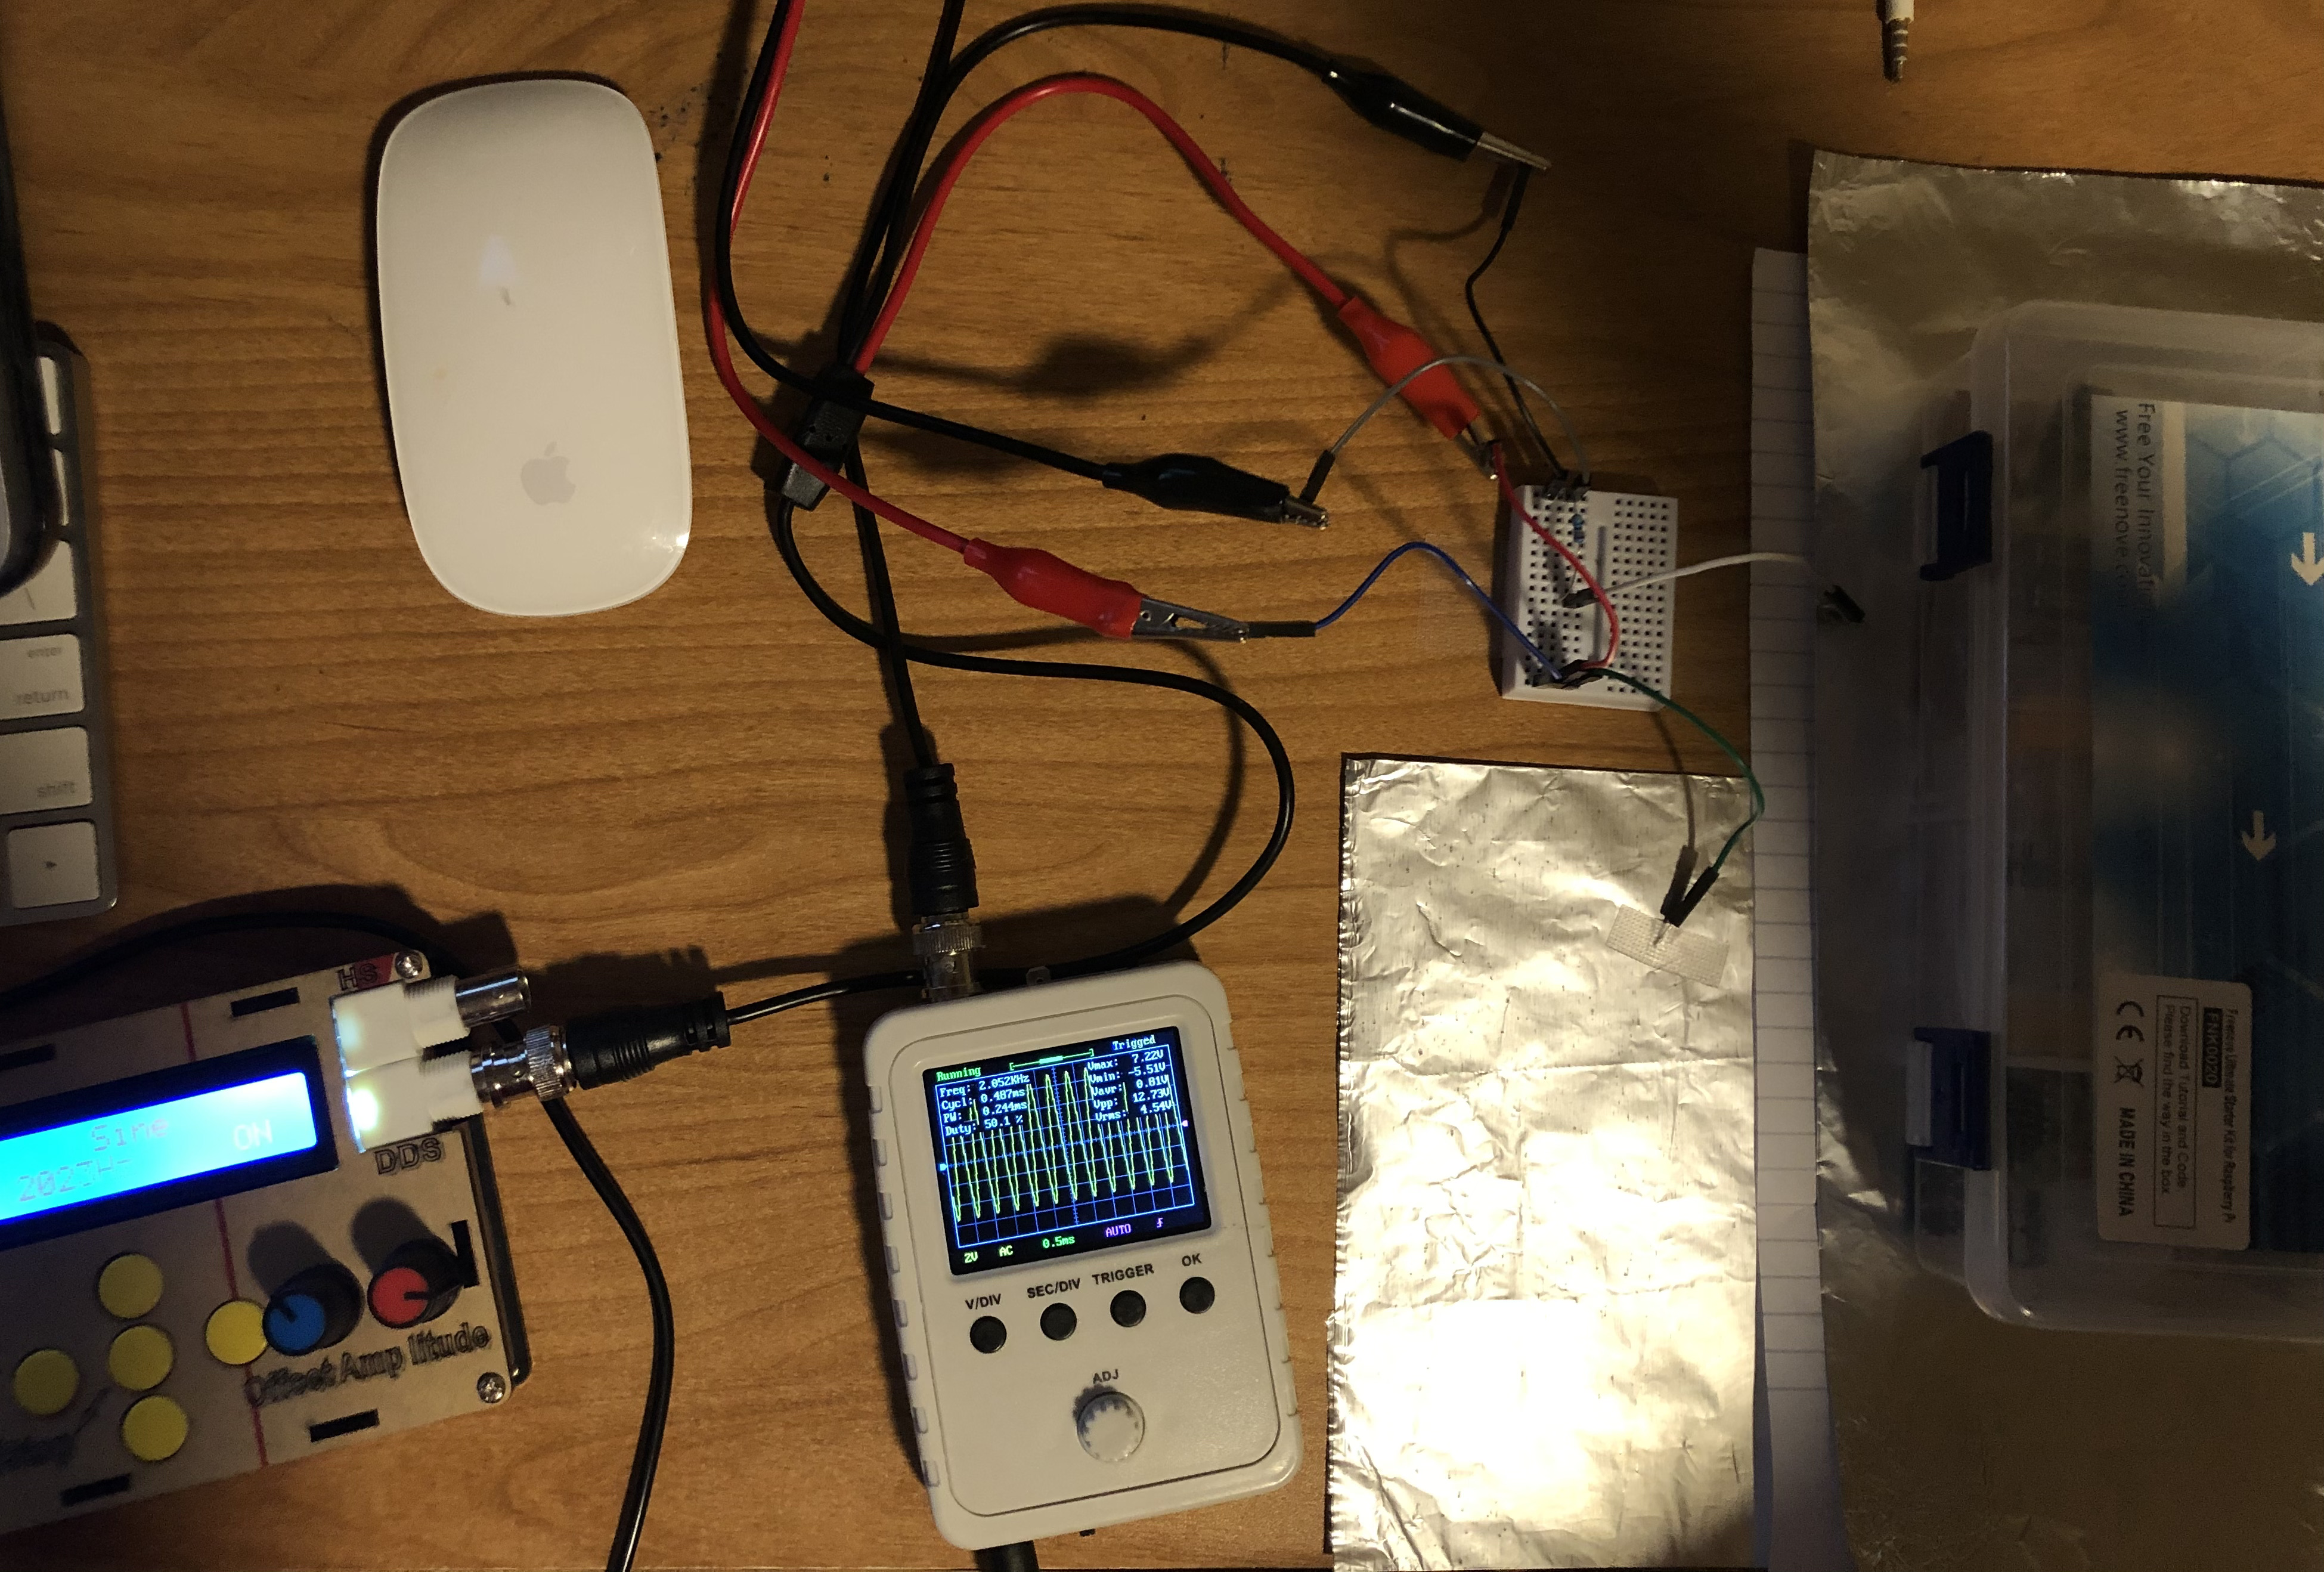
\includegraphics[scale=0.07]{VRC.jpeg}
  \subsection*{\(V_{R}\) Setup}
  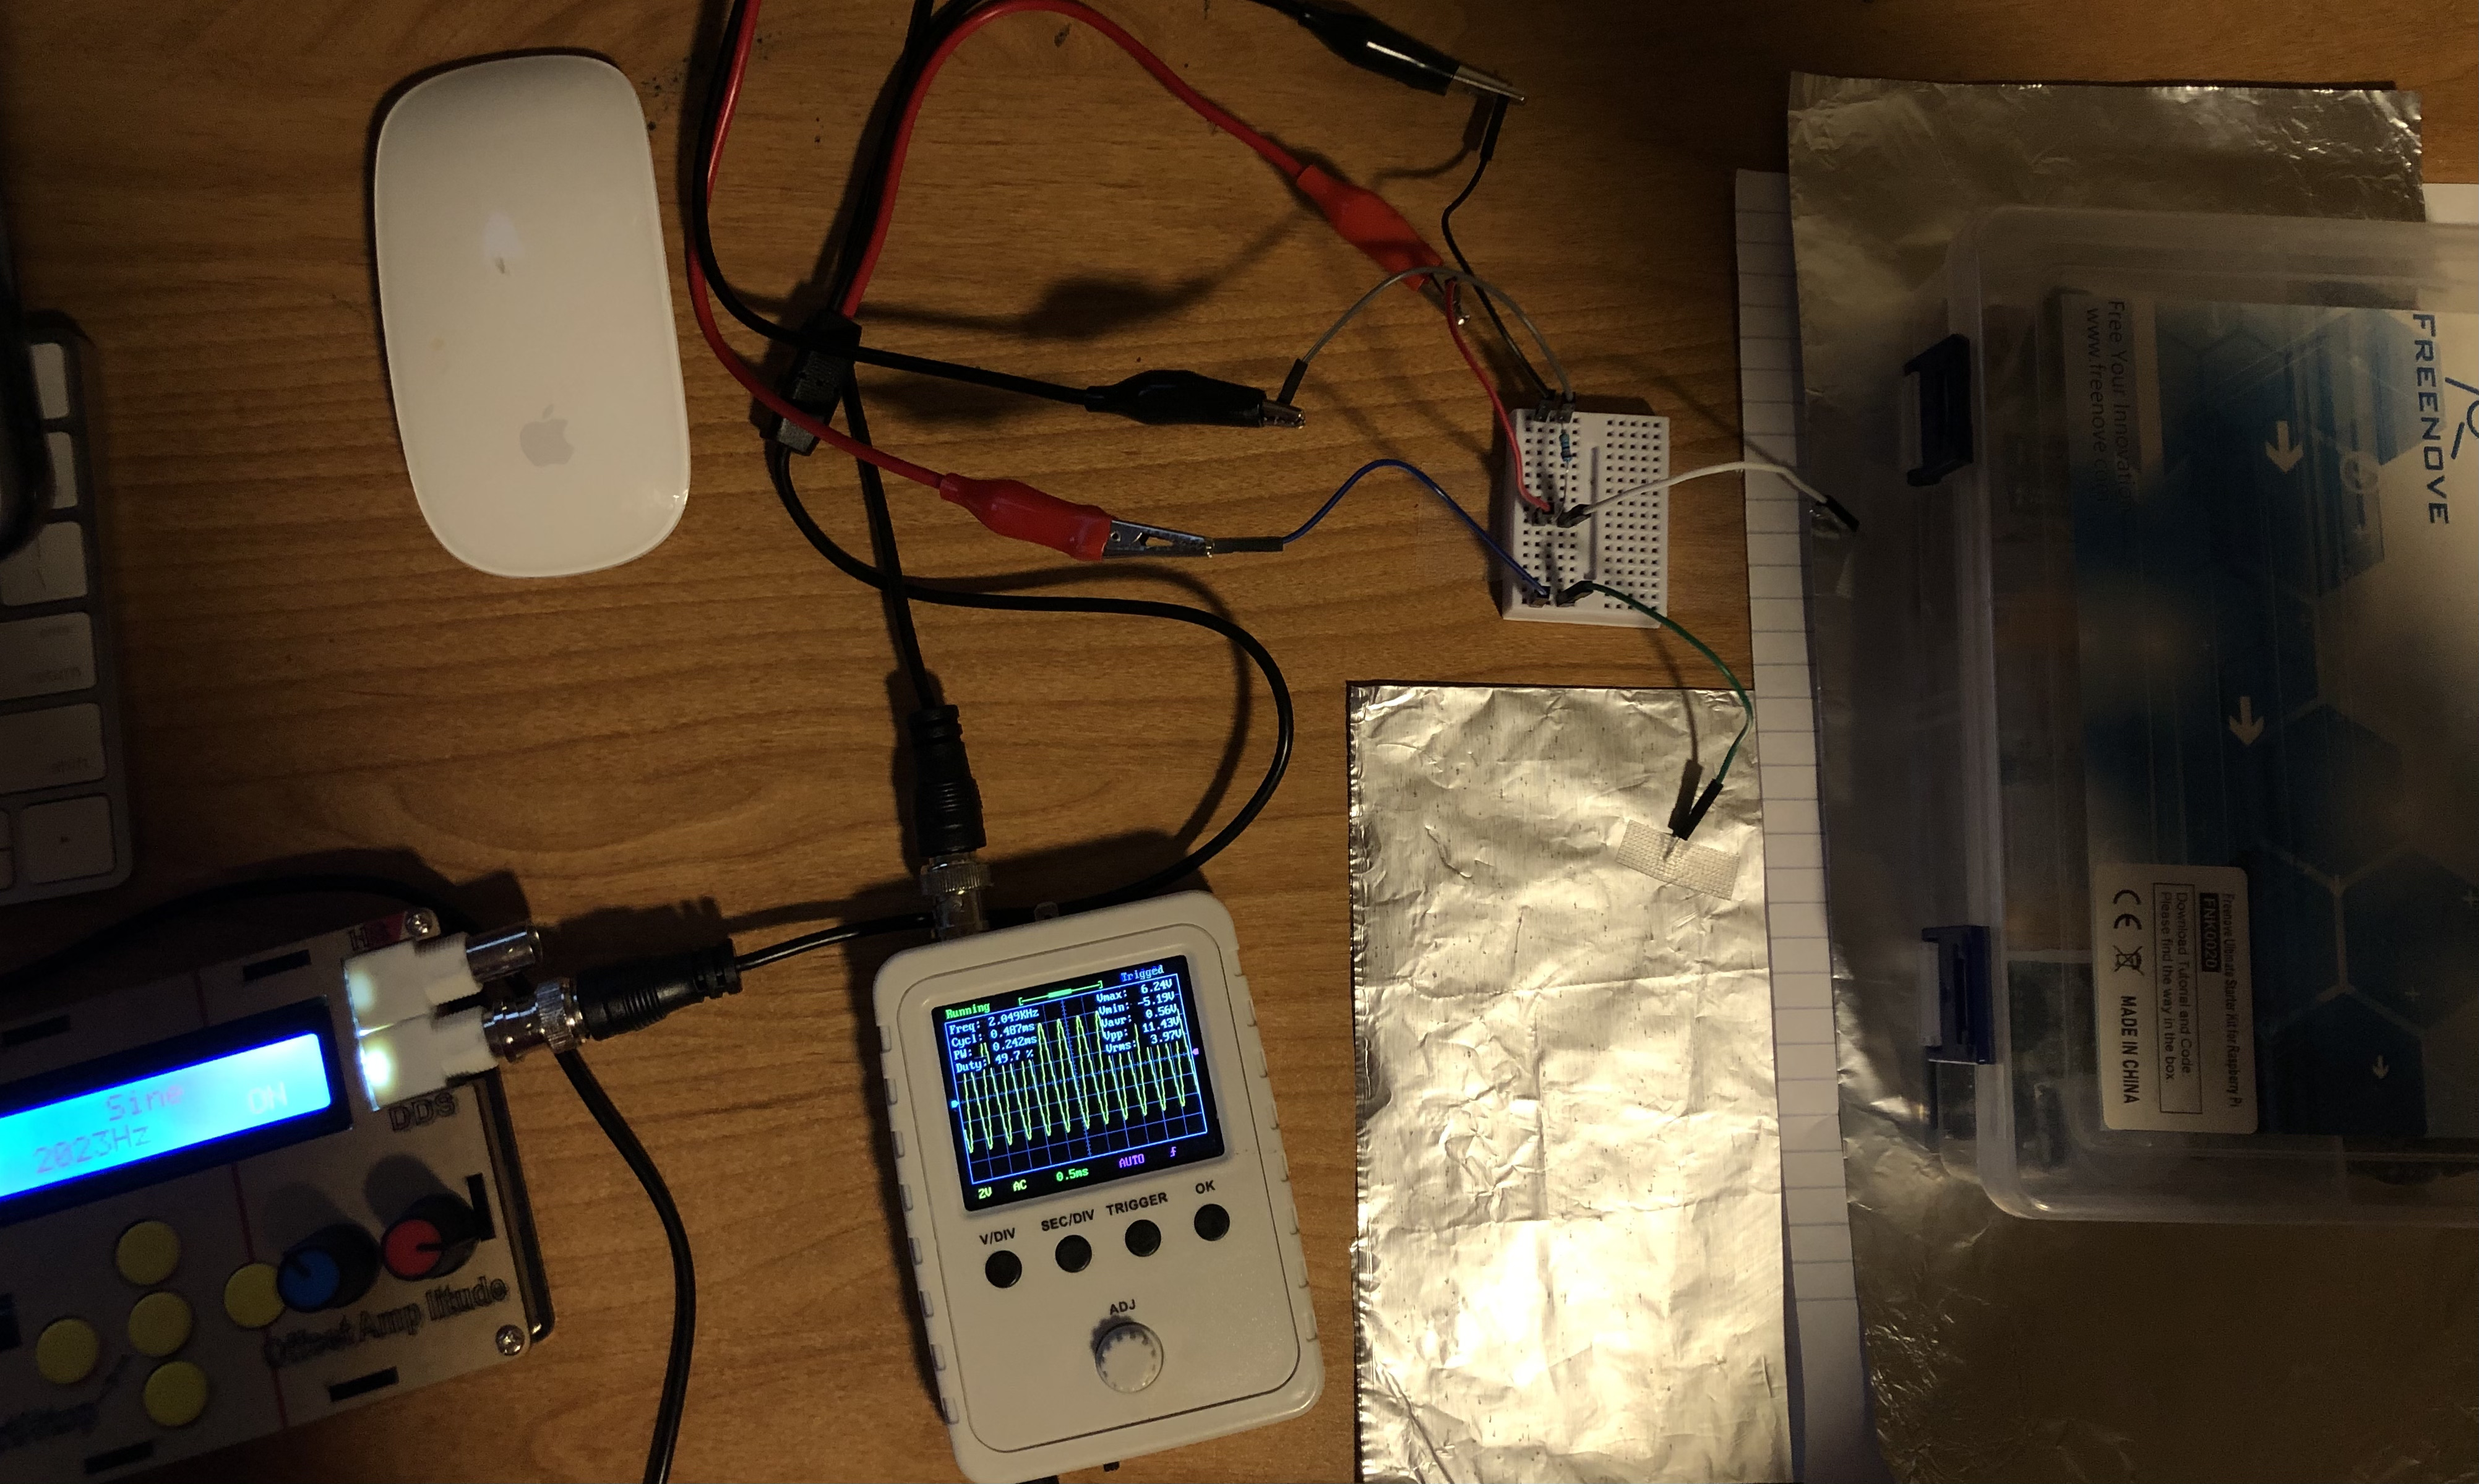
\includegraphics[scale=0.07]{VR.jpeg}
\end{center}

\begin{center}
  \subsection*{Graph 1:}
  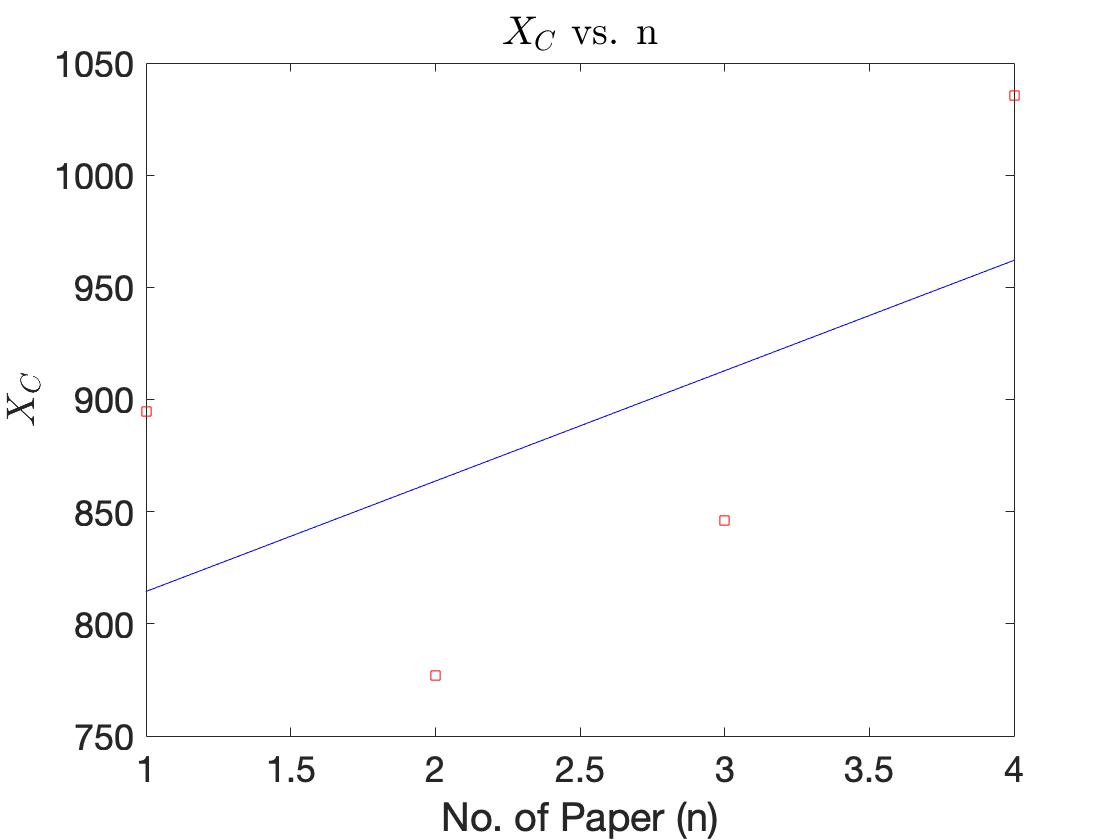
\includegraphics[scale=0.2]{graph1.jpg}
  \subsection*{Graph 2:}
  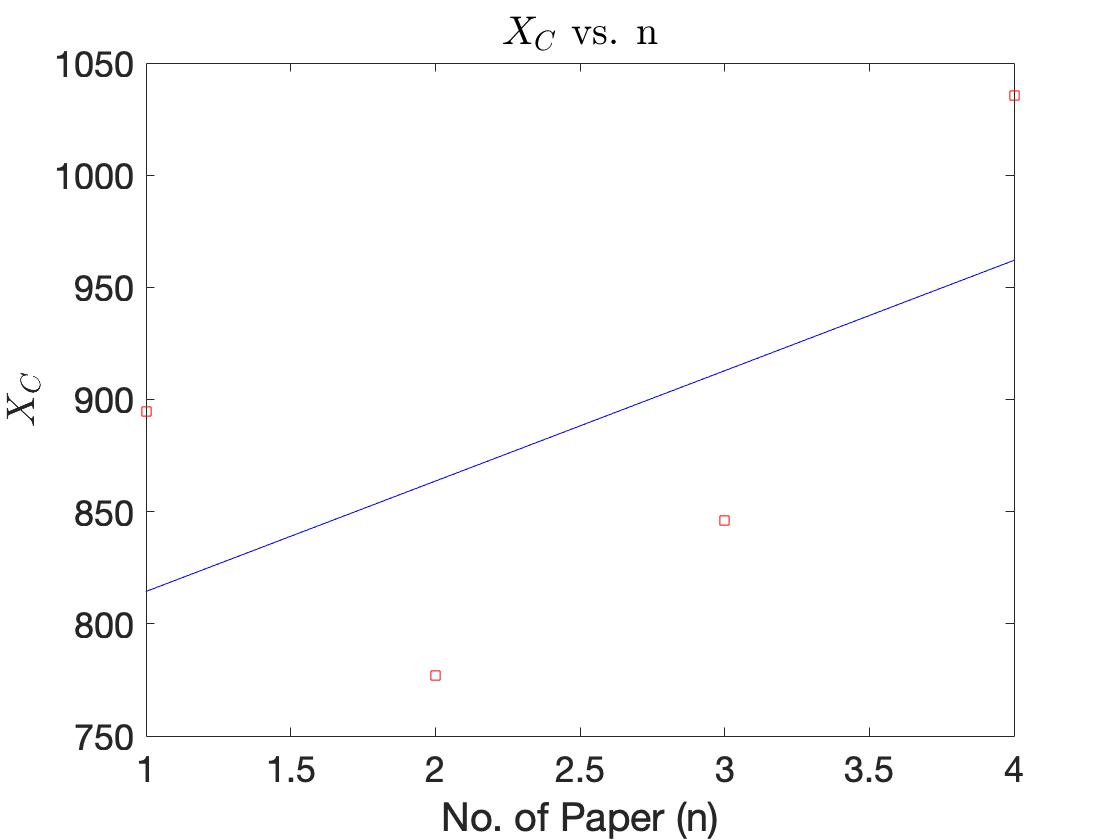
\includegraphics[scale=0.2]{graph2.jpg}
\end{center}
\newpage
\begin{center}
  \begin{enumerate}
    \item What slope do you find for graph 2 and how does it compare to your expectation?
    \begin{itemize}
      \item Slope = 330.36 \(\pm \) 63.22 \(\Omega \)
      \item Expectation = 0.0 \(\pm \) 0.0 \(\Omega \)
    \end{itemize}
    \item What do you think could cause the offset in the fit?
    \begin{itemize}
      \item Mostly from the aluminum foil not being constant and always changing its form.
    \end{itemize}
  \end{enumerate}
\end{center}
\end{document}